
% part 17
\section{Еще один способ написания callback'в\label{sec:part17}}

\subsection{Введение}


В этой главе мы возвратимся к предмету callback'в. Мы изучим 
еще одну технику написания callback'в в Twisted, которая использует 
генераторы. Мы покажем как эта техника работает и сравним с использованием 
<<чистыx>> Deferred'ов. Наконец, мы перепишем один из наших поэтических 
клиентов, используя эту технику. Но сначала, давайте посмотрим на то, 
как работают генераторы, чтобы мы могли увидеть, почему они 
являются кандидатами для создания callback'в.

\subsubsection{Краткий обзор генераторов}

Как вы вероятно знаете, генератор в Python'е - это 
``перезапускаемая функция'', которую вы создаете 
используя выражение yield в ее теле. 
Делая так, функция становится ``генераторной функцией'', 
которая возвращает итератор, который вы можете использовать 
для запуска функции как серии шагов. Каждый цикл 
итератора перезапускает функцию, которая 
продолжает выполняться до тех пор пока не достигнет 
следующего вызова yield.


Генераторы (и итераторы) зачастую используются для представления 
лениво созданных последовательностей значений. Давайте посмотрим 
на пример кода в inline-callbacks/gen-1.py:

\begin{scriptsize}\begin{verbatim}
def my_generator():
    print 'starting up'
    yield 1
    print "workin'"
    yield 2
    print "still workin'"
    yield 3
    print 'done'

for n in my_generator():
    print n
\end{verbatim}\end{scriptsize}


Здесь мы имеем генератор, который создает последовательность 
1, 2, 3. Если вы запустите этот код, то вы увидите, что операторы print в 
генераторе, чередуются с оператором print в цикле, 
проходящему по генератору.


Вы можете сделать этот код более явным 
путем создания самого генератора (inline-callbacks/gen-2.py):

\begin{scriptsize}\begin{verbatim}
def my_generator():
    print 'starting up'
    yield 1
    print "workin'"
    yield 2
    print "still workin'"
    yield 3
    print 'done'

gen = my_generator()

while True:
    try:
        n = gen.next()
    except StopIteration:
        break
    else:
        print n
\end{verbatim}\end{scriptsize}


Генератор --- это просто объект для получения последовательных значений. 
Мы также можем рассмотреть вещи с точки зрения самого генератора:

\begin{enumerate}
\item Функция-генератор не начинает запуск до тех пор, пока она не 
будет вызвана циклом (используя метод next).
\item Запущенный генератор продолжает выполняться до тех пор, пока 
он не возвращается циклу (используя yield). 
\item Когда цикл запускает другой код (подобный оператору print в примере), 
генератор не выполняется.
\item Когда генератор выполняется, цикл не выполняется (блокируется, ожидая возврата генератора).
\item Когда генератор уступает контроль циклу, может пройти произвольное 
количество времени (может быть выполнено произвольное количество кода) до того, 
как генератор запустится снова.
\end{enumerate}


Это очень похоже на то, как работают callback'и в асинхронной системе. 
Мы можем представить, что цикл while - reactor, а 
генератор - серия callback'в, разделенных операторами yield, 
с интересным фактом, что все callback'и разделяют одно и то же 
локальное пространство переменных, и пространство имен сохраняется 
от между всеми вызовами callback'в.


Кроме того, вы можете иметь несколько одновременно активных генераторов 
(посмотрите пример в inline-callbacks/gen-3.py), 
с их чередующимися ``callback'ми'', 
также как вы можете иметь независимые асинхронные задачи, 
запущенные в системе, подобной Twisted.


Хотя, что-то еще пропущено. Callback'и не только вызываются реактором, 
они также получают информацию. Как часть цепочки deferred'а, callback 
либо получает результат, в форме одного Python значения, либо ошибку в 
форме объекта типа Failure. 


Начиная с Python 2.5, функциональность генераторов была 
расширена, что позволило отправлять информацию 
генератору, когда он перезапускается; пример 
inline-callbacks/gen-4.py иллюстрирует это свойство:


\begin{scriptsize}\begin{verbatim}
class Malfunction(Exception):
    pass

def my_generator():
    print 'starting up'

    val = yield 1
    print 'got:', val

    val = yield 2
    print 'got:', val

    try:
        yield 3
    except Malfunction:
        print 'malfunction!'

    yield 4

    print 'done'

gen = my_generator()

print gen.next() # start the generator
print gen.send(10) # send the value 10
print gen.send(20) # send the value 20
print gen.throw(Malfunction()) # raise an exception inside the generator

try:
    gen.next()
except StopIteration:
    pass
\end{verbatim}\end{scriptsize}


В Python 2.5 и выше, оператор yield - выражение, 
которое возвращает значение. А код, который перезапускает генератор, 
может установить это значение, используя метод send вместо next (если 
вы используете next, то значение - None). Более того, 
вы можете генерировать произвольное 
исключение внутри генератора, используя метод throw. И это круто.


\subsection{Встроенные callback'и}

%Given what we just reviewed about sending and throwing values and exceptions into a generator, we can envision a generator as a series of callbacks, like the ones in a deferred, which receive either results or failures. The callbacks are separated by yields and the value of each yield expression is the result for the next callback (or the yield raises an exception and that’s the failure). Figure 35 shows the correspondence:

Взяв за основу то, что мы только что просмотрели об отправке значений и 
генерировании исключений в генераторе, мы можем представить генератор 
как серию callback'в, подобных callback'ам в deferred'е, которые 
получают либо результаты, либо ошибки. callback'и разделены 
yield'ми и значения каждого yield выражения - результат для следующего 
callback'а (или yield генерирует исключение в случае ошибки). 
На рисунке \ref{fig:generator-callbacks1} показано соответствие:
 
% fig35
\begin{figure}[h]
\begin{center}
    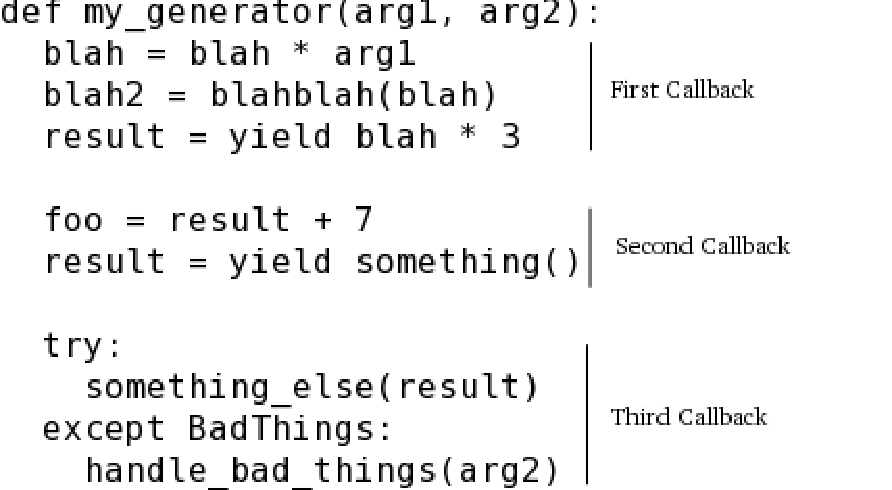
\includegraphics[width=0.5\textwidth]{images/generator-callbacks1.pdf}
    \caption{Генератор как последовательность callback'в\label{fig:generator-callbacks1}}
\end{center}
\end{figure}


Когда серия callback'в соединена вместе в deferred, 
каждый callback получает результат из предыдущего. Это достаточно 
просто сделать и с генератором - просто отправить значение, которое 
имеется от предыдущего запуска генератора, в следующий раз, когда 
вы перезапускаете его. Это кажется немного глупо. Поскольку генератор 
вычислил значение, почему нужно заботится об отправке его назад? 
Генератор может просто сохранить значение в переменной до 
следующего раза, когда она понадобится. Так какой в этом смысл?


Вспомним факт, который мы изучили в главе 13, когда 
callback'и в deferred'е могли возвращать deferred'ы. 
И когда такое происходило, внешний deferred останавливался до тех 
пор, пока внутренный deferred активизировался, и затем 
следующий callback (или errback) в цепочке внешнего deferred'а 
вызывался с результатом (или ошибкой) из внутреннего deferred'а.


Представим, что наш генератор производит объект deferred вместо 
обычного Python значения. Генератор приостановится и это происходит 
автоматически; генераторы всегда приостанавливаются после каждого 
оператора yield до тех пор, пока они явно не перезапустятся. 
Таким образом мы можем приостановить перезапуск генератора до тех пор, 
пока deferred активизируется, в этот момент мы либо отправляем значение 
(если deferred завершился успешно), либо генерируем исключение (если 
deferred завершился с ошибкой). Это могло бы сделать наш генератор 
подлинной последовательностью асинхронных callback'в, что  
являетcя основной идеей в реализации функции inlineCallbacks в twisted.internet.defer. 


\subsubsection{inlineCallbacks}

Рассмотрим теперь пример inline-callbacks/inline-callbacks-1.py:

\begin{scriptsize}\begin{verbatim}
from twisted.internet.defer import inlineCallbacks, Deferred

@inlineCallbacks
def my_callbacks():
    from twisted.internet import reactor

    print 'first callback'
    result = yield 1 # yielded values that aren't deferred come right back

    print 'second callback got', result
    d = Deferred()
    reactor.callLater(5, d.callback, 2)
    result = yield d # yielded deferreds will pause the generator

    print 'third callback got', result # the result of the deferred

    d = Deferred()
    reactor.callLater(5, d.errback, Exception(3))

    try:
        yield d
    except Exception, e:
        result = e

    print 'fourth callback got', repr(result) # the exception from the deferred

    reactor.stop()

from twisted.internet import reactor
reactor.callWhenRunning(my_callbacks)
reactor.run()
\end{verbatim}\end{scriptsize}


Запустите пример, и вы увидите выполнение генератора, 
который по завершению останавливает reactor. Пример иллюстрирует 
несколько свойств функции inlineCallbacks.


Во-первых, 
inlineCallbacks - декоратор, и он всегда декорирует 
генераторные функции, то есть функции, которые используют 
yield. Основная цель inlineCallbacks - превратить генератор 
в серию асинхронных callback'в, согласно тому, как мы 
обсуждали это ранее.


Во-вторых, когда мы вызываем декоратор inlineCallbacks, то 
нам не нужно самим вызывать методы next, send или throw. 
Декоратор сам вызывает эти методы и 
гарантирует, что генератор выполнит весь код (предполагая, 
что в нем не произошло исключения). 


В-третьих, если в генераторе порождается значение, не являющееся 
deferred'ом, то генератор сразу же возвратит себе управление, и 
yield вернет это значение. 


И наконец, если мы порождаем deferred из генератора, 
то генератор не получит управления обратно до тех пор, пока 
deferred не активизируется. После успешного завершения deferred'а, 
управление отдается обратно к генератору, и yield возвращает 
то, что возвратил завершившийся deferred. Eсли 
deferred завершается с ошибкой, то оператор yield генерирует 
исключение. Заметим, что исключение - это просто обычный 
Exception объект, а не объект типа Failure, и мы можем 
поймать его с помощью оператора try/except, обернутого вокруг yield.


В примере мы использовали callLater для активизации  
deferred'в после короткого периода времени. Это удобный 
способ установить неблокирующую задержку в нашу callback 
цепочку, в реальных более сложных програмах, 
мы бы порождали deffered, возвращенный 
некоторой другой асинхронной операцией (например, get\_poetry), 
вызванной из нашего генератора.


Хорошо, теперь мы знаем как запускать функции с декоратором inlineCallbacks, 
но какое значение возвратит 'yield 1'? Ответ - deferred. 
Поскольку мы не можем точно знать, 
когда генератор остановится (он может породить один или 
несколько deferred'ов), декорированная функция сама асинхронная и 
deferred является подходящим возвращяемым значением. 

%Ok, now we know how an inlineCallbacks-decorated function runs, but what return value do you get if you actually call one? As you might have guessed, you get a deferred. Since we can’t know exactly when that generator will stop running (it might yield one or more deferreds), the decorated function itself is asynchronous and a deferred is the appropriate return value. Note the deferred that is returned isn’t one of the deferreds the generator may yield. Rather, it’s a deferred that fires only after the generator has completely finished (or throws an exception).

Поскольку мы заранее не можем сказать, когда 
завершится выполнение генератора, так как он 
может породить несколько deferred'ов, то 
декоратор inlineCallbacks - асинхронная функция 
и deferred - самое подходящее значение в качестве 
возвращаемого значения yield. Заметим, что для возвращаемого  
deferred'а, генератор не может вызвать yield. Заметим, что 
возвращаемый генератором deferred не порождается оператором yield. 
Напротив, этот deferred может активизироваться только после того как 
генератор полностью завершился (или выкинул исключенение). 

%If the generator throws an exception, the returned deferred will fire its errback chain with that exception wrapped in a Failure. But if we want the generator to return a normal value, we must “return” it using the defer.returnValue function. Like the ordinary return statement, it will also stop the generator (it actually raises a special exception). The inline-callbacks/inline-callbacks-2.py example illustrates both possibilities.

Если генератор выкидывает исключение, 
то возвращаемый deferred активизирует свою 
цепочку errback с исключением, обернутым в Failure. 
Но, если вы хотите, чтобы генератор возвращал 
обычное значение, вы должны использовать функцию 
defer.returnValue. Подобно обычному оператору return, 
он также остановит генератор (в действительности, он 
генерирует специальное исключение). Пример 
\href{http://github.com/jdavisp3/twisted-intro/blob/master/inline-callbacks/inline-callbacks-2.py#L1}{inline-callbacks/inline-callbacks-2.py} иллюстрирует 
обе возможности.

\subsection{Клиент 7.0}

Давайте включим inlineCallbacks в новую версию нашего поэтического 
клиента. Код находится в twisted-client-7/get-poetry.py. 
Можно сравнить с кодом клиента 6.0 в twisted-client-6/get-poetry.py. 
Изменения в основном коснулись poetry\_main:

\begin{scriptsize}\begin{verbatim}
def poetry_main():
    addresses = parse_args()

    xform_addr = addresses.pop(0)

    proxy = TransformProxy(*xform_addr)

    from twisted.internet import reactor

    results = []

    @defer.inlineCallbacks
    def get_transformed_poem(host, port):
        try:
            poem = yield get_poetry(host, port)
        except Exception, e:
            print >>sys.stderr, 'The poem download failed:', e
            raise

        try:
            poem = yield proxy.xform('cummingsify', poem)
        except Exception:
            print >>sys.stderr, 'Cummingsify failed!'

        defer.returnValue(poem)

    def got_poem(poem):
        print poem

    def poem_done(_):
        results.append(_)
        if len(results) == len(addresses):
            reactor.stop()

    for address in addresses:
        host, port = address
        d = get_transformed_poem(host, port)
        d.addCallbacks(got_poem)
        d.addBoth(poem_done)

    reactor.run()
\end{verbatim}\end{scriptsize}


В новой версии генератор get\_transformed\_poem с декоратором 
inlineCallbacks отвечают за скачивание поэмы и ее 
преобразование (через трасформирующий сервер). Поскольку 
обе операции асинхронные, мы порождаем (оператором yield) 
deferred и затем явно ждем результат. Так же как и клиент 6.0, 
если преобразование завершилось с ошибкой, то поэма не 
меняется. Заметим, что мы можем использовать операторы 
try/except для управления асинхронными ошибками внутри 
генератора.


Мы можем проверить новый клиент так же как и раньше. 
Сначала запустим трансформирующий сервер:

\begin{scriptsize}\begin{verbatim}
python twisted-server-1/tranformedpoetry.py --port 10001
\end{verbatim}\end{scriptsize}

Затем запустим несколько поэтических серверов:

\begin{scriptsize}\begin{verbatim}
python twisted-server-1/fastpoetry.py --port 10002 poetry/fascination.txt
python twisted-server-1/fastpoetry.py --port 10003 poetry/science.txt
\end{verbatim}\end{scriptsize}

Теперь можно запустить новый клиент:

\begin{scriptsize}\begin{verbatim}
python twisted-client-7/get-poetry.py 10001 10002 10003
\end{verbatim}\end{scriptsize}

Попробуйте отключить один или несколько серверов, для 
того, чтобы посмотреть как клиент управляет ошибками.


\subsection{Обсуждение}

Подобно объекту Deferred, функция inlineCallbacks дает 
новый способ организации наших асинхронных callback'в. 
Так же как и с deferred'ми, inlineCallbacks не меняет 
правила игры. Наши callback'и запускаются 
один за раз и вызываются реактором. Мы можем убедиться 
в этом, распечатав traceback из внутреннего callback'а, 
так, как это сделано в примере 
\href{http://github.com/jdavisp3/twisted-intro/blob/master/inline-callbacks/inline-callbacks-tb.py#L1}{inline-callbacks/inline-callbacks-tb.py}. Запустите пример, и вы увидите 
traceback, начинающийся с reactor.run(), завершающийся 
нашим callback'м и несколько вспомогательных функций 
между ними.


Мы можем адаптировать рисунок \ref{fig:deferred-12}, который 
объясняет как один callback в deferred'е возвращает другой deferred, 
чтобы показать, что случается, когда генератор 
inlineCallbacks порождает deferred (при помощи yield). 
Посмотрите на рисунок \ref{fig:inline-callbacks1}.

\newpage

% fig36
\begin{figure}[h]
\begin{center}
    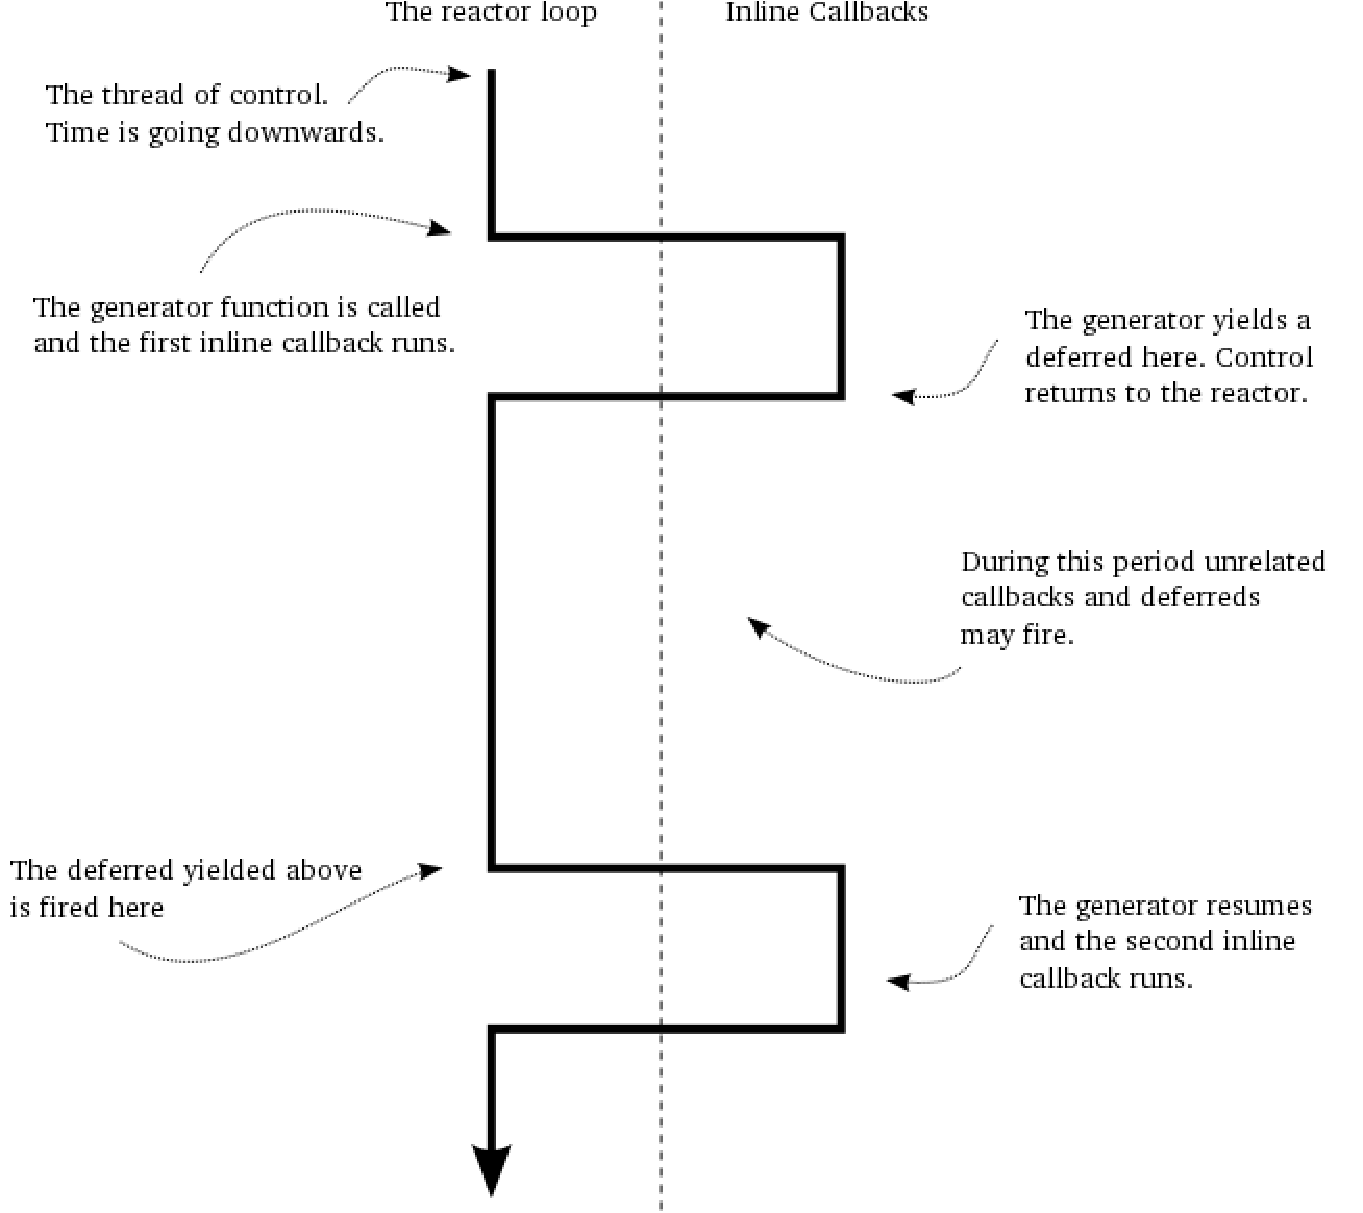
\includegraphics[height=0.5\textheight]{images/inline-callbacks1.pdf}
    \caption{Поток выполнения в функции inlineCallbacks\label{fig:inline-callbacks1}}
\end{center}
\end{figure}


Оба рисунка иллюстрируют одну и ту же идею: 
одна асинхронная операция ожидает другую.


Поскольку inlineCallbacks и deferred'ы решают много 
идентичных проблем, что лучше выбрать? Существует 
несколько преимуществ inlineCallbacks:

\begin{itemize}

\item Посколько callback'и разделяют пространство 
    имен, не нужно использовать дополнительное состояние.

\item Порядок callback'в легче просматривается, так как они 
    выполняются сверху вниз.
    
\item Без объявлений функций для индивидуальных 
    callback'ов и явным потоком управления в общем случае получается 
    меньше текста.

\item Ошибки обрабатываются с помощью оператора try/except.

\end{itemize}

Также возможны следующие проблемы:

\begin{itemize}
%    * The callbacks inside the generator cannot be invoked individually, which could make code re-use difficult. With a deferred, the code constructing the deferred is free to add arbitrary callbacks in an arbitrary order.

\item Callback'и внутри генератора не могут быть вызваны 
    индивидуально, что делает сложным переиспользование 
    кода. С deferred'ми, при конструировании кода, можно  
    просто добавить произвольные callback'и в 
    произвольном порядке.


%    * The compact form of a generator can obscure the fact that an asynchronous callback is even involved. Despite its visually similar appearance to an ordinary sequential function, a generator behaves in a very different manner. The inlineCallbacks function is not a way to avoid learning the asynchronous programming model.

\item Компактная форма генератора делает неявным 
    факт использования асинхронных callback'ов. Несмотря на 
    визуальное сходство с обычными последовательными 
    функциями, генератор выполняется отличным образом. 
    Функция inlineCallbacks - не способ избежать 
    изучения асинхронной модели программирования.

\end{itemize}


Также как и с любой другой технологией, 
практика обеспечит необходимым опытом для правильного выбора между 
callback'ми и генератором, обернутым в декоратор inlineCallbacks.


\subsection{Резюме}

В этой главе мы изучили декоратор inlineCallbacks и о том, как 
он позволяет нам выражать последовательность 
асинхронных callback'ов в форме Python генератора.


В следующей главе мы изучим технику управления 
множеством ``параллельных'' асинхронных операций.


\subsection{Упражнения}

\begin{enumerate}

\item Почему название функции inlineCallbacks во 
    множественном числе?

\item Изучите реализацию функции inlineCallbacks и ее 
    управляющую функцию \_inlineCallbacks. Подумайте над 
    фразой ``дьявол в деталях''.

\item Сколько callback'в в генераторе с N 
    операторами yield, предполагая, что нет циклов и 
    условных операторов (if)? 


%   4. Poetry client 7.0 might have three generators running at once. Conceptually, how many different ways might they be interleaved with one another? Considering the way they are invoked in the poetry client and the implementation of inlineCallbacks, how many ways do you think are actually possible?

\item Поэтический клиент 7.0 может иметь три генератора, 
    запущенных одновременно. Концептуально, сколько различных 
    способов чередования их выполнения? Учитывая способ, 
    которым они вызываются в поэтическом клиенте и 
    реализацию inlineCallbacks, как вы думаете, сколько 
    способов действительно возможно?

\item Переместите callback got\_poem в клиент 7.0 внутрь генератора.

%   6. Then move the poem_done callback inside the generator. Be careful! Make sure to handle all the failure cases so the reactor gets shutdown no matter what. How does the resulting code compare to using a deferred to shutdown the reactor?

\item Переместите callback poem\_done внутрь генератора. 
    Будьте внимательны! Убедитесь, что управляете всеми 
    случаями ошибок, чтобы reactor завершился не смотря 
    ни на что. 

\item Генератор с оператором yield внутри цикла while 
    представляет собой бесконечный цикл. Что представляет собой 
    генератор с декоратором inlineCallbacks?

\end{enumerate}



